\documentclass[conference]{IEEEtran}
\IEEEoverridecommandlockouts
% The preceding line is only needed to identify funding in the first footnote. If that is unneeded, please comment it out.
\usepackage{cite}
\usepackage{amsmath,amssymb,amsfonts}
\usepackage{algorithmic}
\usepackage{graphicx}
\usepackage{textcomp}
\usepackage{xcolor}
\def\BibTeX{{\rm B\kern-.05em{\sc i\kern-.025em b}\kern-.08em
    T\kern-.1667em\lower.7ex\hbox{E}\kern-.125emX}}
\begin{document}

% \title{Development of Online Judge Using Contestant PC As Worker of Autograder}
\title{Development of Autograder For Competitive Programming Using Contestant PC As Worker}

\author{\IEEEauthorblockN{Jauhar Arifin}
\IEEEauthorblockA{School of Electrical Engineering and Informatics} \\
Bandung Institute of Technology\\
Bandung, Indonesia \\
jauhararifin10@gmail.com
\and
\IEEEauthorblockN{Riza Satria Perdana}
\IEEEauthorblockA{School of Electrical Engineering and Informatics} \\
Bandung Institute of Technology\\
Bandung, Indonesia \\
riza@informatika.org}

\maketitle

\begin{abstract}
Competitive programming is a computer science competition where the contestants compete to solve computer science problems by writing a program which satisfies the problem constraints.
Autograder is used to grade contestant solutions automatically in real-time. Usually autograder is deployed in many computers to increase grading performance. In this work, contestant computers are used as worker to run autograder. By using contestant computers as worker, the number of worker will proportional to the number of contestant submissions, thus increasing grading performance. Every contestant computers have different specification and can affect grading fairness. To keep grading fairness, contestant's solution and jury's solution executed in contestant worker and compared to check whether contestant's solution satisfies problem constraints. This work tested by simulating grading process in contestant computers. The testing result indicates that using contestant computers as worker gives performance improvement in the grading process.
\end{abstract}

\begin{IEEEkeywords}
competitive programming, online judge, autograder.
\end{IEEEkeywords}

\section{Introduction}

Competitive programming is one of the most popular competition in computer science field. In competitive programming competition, contestants are asked to solve computer science problems correctly and as fast as possible. Some institute and organization often organize competitive programming competition periodically. Some big companies like Google and Facebook organize competitive programming competition annually. Competitive programming competition supported by online judge system. Usually, online judge system is a web based application where contestants can read the problems, create clarifications, submit their solution, and watch the scoreboard. Currently, the most popular online judge are Codeforces, URI Online Judge \cite{uriojpaper}, Uva, and SPOJ.

In order to grade contestant submissions, online judge system has a subsystem called autograder. Contestant submissions which are source code in certain programming language will be graded by autograding system by compiling the program and executes compiled program using test-cases that have been prepared by juries or problem setter. According \cite{jordanioi}, this grading method is called black-box grading. By using autograding system, the grading process can be done automatically and juries don't have to evaluate contestant submissions manually. In order to increase the number of contestant submissions in certain amount of time, juries usually deploy autograder in many computers. In order to run autograder in many computers, the juries need to prepare many computers with the same spesification to keep the fairness of grading process.

Currently, almost every competitive programing competition use online judge system to support the competition and use many computers to run autograder in order to improve grading performance. Every computers that run autograder are called worker. Grading performance is defined as the number of submissions graded in certain amount of time. Even though autograder deployed in many computers, the grading performance often not enough to evaluate contestant solutions in real-time because the number of contestants is increasing. Furthermore, the number of computer to deploy autograder affect the procurement cost that juries need to be incurred. Therefore, new grading system is needed to increase grading performance without increasing procurement cost that need to be incurred.

When competing in competitive programming competition, the contestants usually use their personal computer to write the solutions. Every contestant computers usually have sufficient specification to compile and execute contestant submissions. Therefore, contestant computers have ability to run autograder program and evaluate contestant submissions.

\section{Related Work}

There are some popular online judge system that have been used to organize competitive programming competition. Some online judge offer another additional features like discussion forum, training gate and rating system. Nowadays, most of online judge deployed as web application and use specific computer to grade contestant submissions. There are many types of competitive programming competition rules. Most of online judge only support a specific competition rules.

One of the most popular competitive programming competition is ACM-ICPC competition where the competition uses ICPC rules. In ACM-ICPC competition, contestants compete in group of three people. Every group have the same amount of problem to solve, and the score is determined by the number of solved problem and time penalty. There are many online judges that support this competitive programming rules. The most popular online judge that support this type of competition is DOMJudge. DOMJudge is very popular because it has many usefull feature, easy to use and open source.

Currently, most of online judge use autograder to evaluate contestant submissions. According to \cite{danutamalms}, autograder is a system that compiles, executes and evaluate source code. Evaluates source code manually takes three minutes while using autograder only need ten seconds. By using autograder, contestants can receive grading feedback faster and reduce the work that need to be done by juries. Basically, the autograder evaluate the source code by compiles the source code, and executes the compiled program using predefined test-cases. The output of contestant's solution program compared to the predefined test-case and then graded. This evaluation method is called black-box grading \cite{jordanioi}.

We need to consider security aspect when developing autograding system. Competitive programming contestants might submit source code that contain dangerous code. According to \cite{wasikojsurvey}, there are several attacks that can be made by contestants, such as submitting compile bomb code, submitting code that destroy autograding environment, and submitting code that access forbidden computer's resource. In order to prevent such things, autograding system must execute contestant's code in isolated environment called sandbox.

There are several ways to create isolated environment such as using virtual machine and containerization. By using virtual machine, one can create isolated operating system inside host computer. Virtual machine uses hypervisor to emulate computer hardware and run its own operating system. In Linux based operating system, there is a feature called KVM that make it possible to create hypervisor as a process in Linux \cite{wfeltervmcontainer}. We can use virtual machine to isolate the execution of contestant's code. However, by using virtual machine, we need to boot a new operating system each time we evaluate contestant's subission. This booting process takes so much computer's resource and reduces grading performance.

Another way to create isolated environment is by using container. Container is different from virtual machine. Container Container gives isolation in software level wihout hypervisor \cite{merkeldocker}. By using container, we can isolate process execution without boot a new operating system. Container works by using some Linux features such as chroot, namespace and cgroup. By using chroot, we can isolate filesystem of Linux process \cite{lessardchroot}. Container uses Linux feature called cgroup to limit process resources. By using cgroup, we can limit memory usage, CPU usage and disk IO usage of running process \cite{wfeltervmcontainer}. In order to hide other process, user, and network from a running process, container uses a Linux feature called namespace. By using namespace, we can isolate a Linux process from other process, so the running process not aware of the existance of other process. Instead of virtual machine, most of autograding system use container to isolate grading process. This method is used because it is more lighter and faster than virtual machine. 

\section{Methodology}

\subsection{Time and Memory Measurement}

In competitive programming competition, every problems has time and memory constraints. Contestants are asked to solve the problem by writing program that satify the constraints. According to ICPC rules, when contestant's solution exceeds the problem constraints, the solution is rejected and the contestant get time penalty. Thus, autograding system need to tell whether contestant's solution exceeds the constraints or not. The probem is, every computer has different performance when executing a program. The same program might run faster in one computer and slower in another computer. Currently, most of online judge system uses identical computer to evaluate contestant submissions. By using identical computer, the same program expected to run at the same duration and consume the same amount of memories.

Contestant computers have different specification and performance. We cannot force the contestants to have identical computer. Thus, we need new time and memory measurement method. The performance of a computer is determined by its specifications such as CPU clock speed and operating system. We can tell the computer performance by its specifications. However, besides CPU clock speed and operating system, there are so much other factors that affect computer performance such as temperature, cache size, the program itself, and many other factors. Thus, determining computer performance by its specification is very hard and not feasible to do.

\begin{equation}\label{tolerance-factor}
R_{contestant} < (1 + \gamma) \times R_{jury}
\end{equation}

In this work, we compare contestant's solution and jury's solution. Contestant's solution considered satisfying the problem constraints when the memory and CPU usage of contestant's solution not exceeding jury's solution. Sometimes, contestant solution's memory or CPU exceeds jury's solution a little bit because the implementation is different. We add tolerance factor ($\gamma$) to tolerate this problem. Contestant's solution is considered satifying problem constraints when the Equation \ref{tolerance-factor} is fulfilled. When evaluating contestant's solution, the worker compiles and executes contestant's solution and jury's solution. After executes the solutions, the worker compares the memory and CPU usage of the execution and determine whether the contestant's solution satisfy problem constraints. 

\subsection{Load Balancing}

We need to distribute grading jobs to worker evenly in order to increase grading performance. There are several load balancing method that we can use to distribute grading jobs evenly. The easiest way to distribute the jobs is by making each contestants to grade their own submissions. In this work, we didn't use this method because this method creates security vulnerabilites.

The other way distribute grading jobs is by using push-based load balancing method. In push-based load balancing, the online judge server choose the worker to do the grading jobs. By using this method, every contestant doesn't know which submission they grade, thus can increase system security. To improve system security, we can also grade every submission multiple times. In order to implement this method, we need the status of all workers. This method is pretty hard to implement because we need to poll the worker status periodically and choose the best worker to evaluate the contestant submissions.

\begin{figure}[htbp]
\centerline{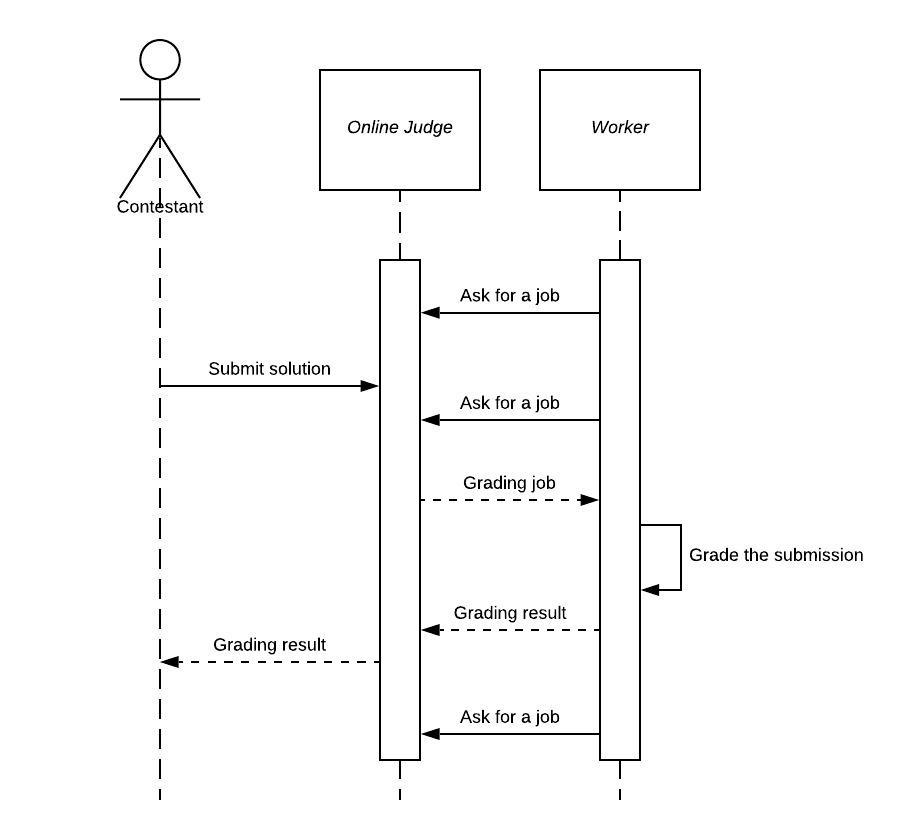
\includegraphics[width=0.4\textwidth]{images/paper-pull-based-load-balancing.jpeg}}
\caption{Pull-based Load Balancing.}
\label{pull-based-load-balancing}
\end{figure}

In this work, we use pull-based load balancing method. By using this method, we don't have to poll the worker status periodically. The worker will poll the jobs from server periodically and evaluate them when the there is a job that ready to be evaluated. To improve the system security, we grade every submission multiple times. We define a grading size of the system as the number of times we need to grade each submission. Fig. \ref{pull-based-load-balancing} depicts this method mechanism. This work is easier to implements than push-based load balancing method and has the same advantages.

\subsection{Evaluating Submission In Isolated Environment}

\begin{figure}[htbp]
\centerline{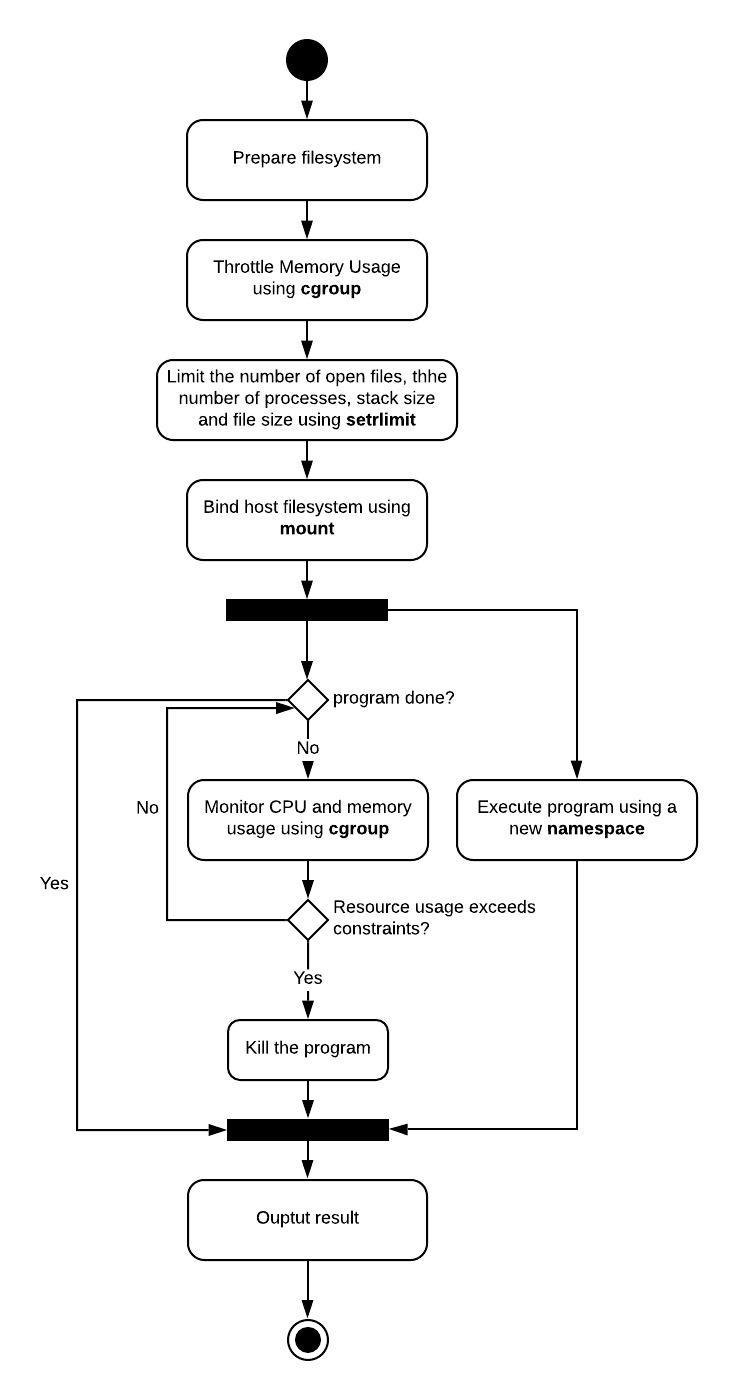
\includegraphics[width=0.4\textwidth]{images/paper-sandbox-activity.jpeg}}
\caption{Sandbox Activity Diagram.}
\label{paper-sandbox-activity}
\end{figure}

In order to isolate the evaluation process, we use containerization method. We compile and execute contestant's submission inside lightweight container. This container is created by using several Linux features and system calls such as cgroup, namespace, chroot and setrlimit. We use cgroup to monitor and limit the CPU and memory consumption of running process. The worker kills the program when the CPU or memory usage is exceeding the limit. In order to isolate the host's user, process and network, we use Linux feature called namespace. By using namespace, the processes inside isolated environment will not aware of any process, user or network in the outside of its own environment. In order to isolate filesystem of a process, we use chroot system call. Beside isolating the filesystem, we also need to bring some files from host environent into the isolated environment. We bring some of host filesystem into the isolated environment by using mount system call. We also limit the process limit by using setrlimit system call. By using setrlimit system call, we limit some process resources such as the number of child processes, the stack size, the number of open files and the size of file created by that process. Fig. \ref{paper-sandbox-activity} depicts how isolated environment is created.

\subsection{Program Compilation}

In order to evaluate contestant's submissions, we need to compile and execute the submitted source code. To compile the source code, we need a specific compiler. Every worker should has the same version of compiler. The same compiler with different version can produces different output. In order to keep the fairness of grading process, we need to distribute the same version of compiler to all workers in the system. In this work, we distribute the compiler in the autograder program to every workers. Every worker compiles the source code inside an isolated filesystem that has been installed with the same version of compilers.

\subsection{Obtaining Problem Test-cases}

Every worker needs test-cases to evaluate contestant solutions. A test-case is a pair of text file that contains input and output of the problem. Usually, the test-case files are generated by test-case generator that created by problem setters. The worker evaluates the contestant solution by executing the solution using the input test-case and compare the output with the output test-case. In order to evaluate the contestant solutions, we need to bring the problem testcases into the worker. To bring the test-cases into the worker is not easy because the test-case file can be a very large file and confidential.

In this work, we don't transfer the raw test-case files to all the workers. Transfering raw test-case files needs a huge bandwidth and can reduce grading performance. Instead of transfering raw test-case file, we transfer the test-case generator program to generate test-case files. The worker receive test-case generator source code from the server and compiles it. The compiled test-case generator program then executed to generates input test-case. The worker uses jury's solution to generates output test-case files. The worker also needs checker program to compare contestant's output with jury's output. The checker program receive contestant's output and jury's output as its input and gives the verdict of the submission.

In order to hide the test-case information, we encrypt the test-case generator program and the generated test-case files. Even though the test-case is encrypted, the contestants might decrypt it if they know the encryption key. The contestant can attacks the autograder program using reverse engineering technique to obtain the encryption key. In this work, we didn't handle this problem. Further research are needed to solve this problem.

\subsection{Handling Reverse Engineering Attacks}

Because the autograder programs are deployed in the contestant computers, the contestants can do everything to the program. The contestant can attacks the autograder program in their computer. There are many kind of attacks that the contestant can do such as changing the compiler program, sending the false verdict to the server and refuse to grade other contestant submission. In this work, we didn't handle this kind of attacks, but there is a way to handle this kind of attacks.

We can prevent a contestant to refuse do the grading process by monitoring the grading process. When we find out that there is a worker that not asks for job for a long time or not sends the grading result for a long time, we can tell that there is a contestant that attacks the autograder program in their computer. Then, we can warn or disquafy the contestant for attacking the autograder program.

By grading every submission multiple times, we can prevent a worker from being atacked that cause it gives wrong verdict after grading. When we grade a submission multiple times and there is a contestant that attacks the autograder in their computer, we can tell by investigating the grading result. If the grading result of a worker is different from the rest of workers, we can tell that the contestant attacks the autograder program in that worker. Then, we can warn or disquafy that contestant for attacking the autograder program.

There are many more type of attacks that we didn't handle in this work such as stealing jury's solution, other contestant's solution and test-case generator. Even though we didn't handle some type of attacks, this system can still works in several competition such as ACM-ICPC. In ACM-ICPC, every team is given a computer by the juries to solve the problems. The juries can install autograder program inside contestant's computer using root user and not giving the root access to the contestant. By using this mechanism, the contestant can't attacks the autograder program inside their computer.

\section{Implementation}

We named this system UGrade and implement this by develop five programs, i.e., UGServer, UGDesktop, UGCtl, UGJob and UGSbox. UGServer handle everything related to competition such as authentication, contest creation, problem creation, etc. We can consider UGServer as a server of all the workers in the system. UGServer stores all the problems, submissions and the grading results. We develop UGServer using Python with Django and use GraphQL for the API. We use Django because of its ease of use.

\begin{figure}[htbp]
\centerline{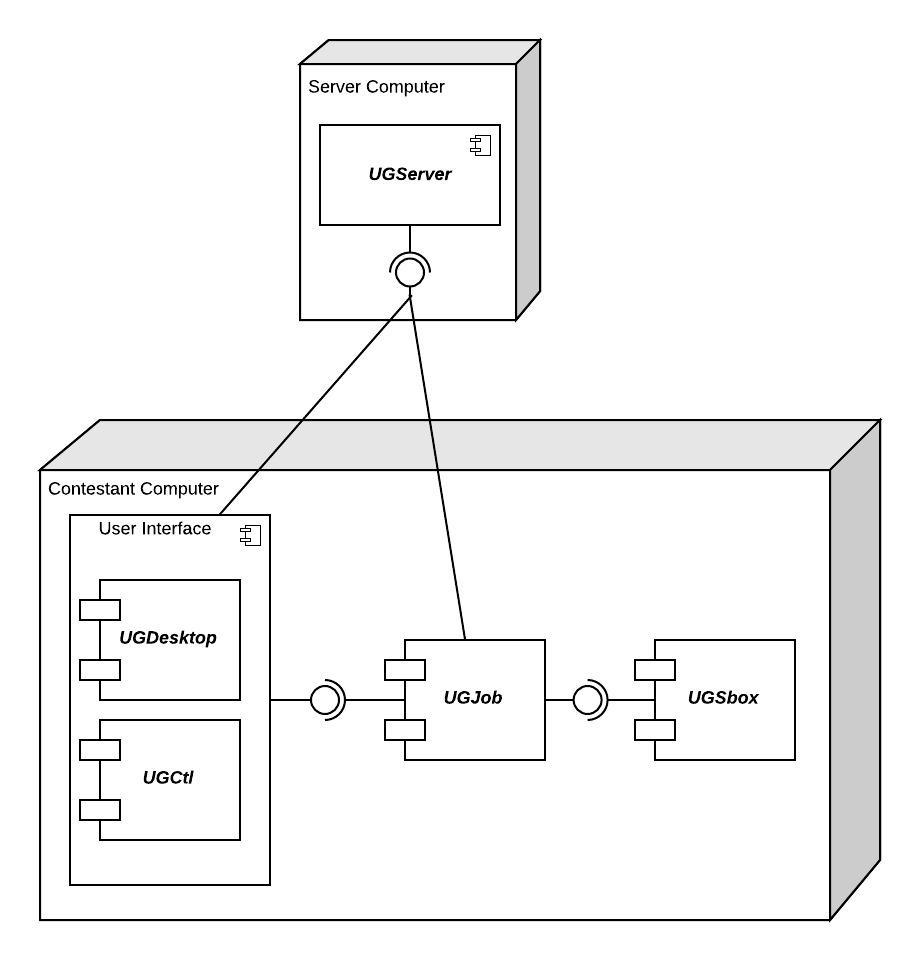
\includegraphics[width=0.4\textwidth]{images/paper-component.jpeg}}
\caption{Component Diagram of UGrade}
\label{component}
\end{figure}

To create isolated environment, we create sandbox utility program called UGSbox. By using UGSbox, one can execute a program inside an isolated environment and limit its resources. We develop UGSbox using Golang because its ease of use. UGSbox is used by autograder program to compiles and executes the program for grading process.

In this work, we named the autograder program as UGJob. UGJob asks UGServer for a job and do the grading process. UGJob uses UGSbox to compiles and executes the source code it receives from UGServer. We develop UGJob using Golang because it ease of use. The UGJob is deployed in every contestant computers. Every installation of the UGJob is equipped with the same compiler to improve the fairness of grading process.

The contestants can interact with the system using user interface programs, e.g., UGDesktop and UGCtl. UGDesktop is a graphical user interface program to interact with this system. Every contestant use UGDesktop to read the problem and submit their solutions. UGDesktop will execute UGJob periodically to grade the available job in the server. UGCtl is a text-based user interface program to interact with this system. Basically, UGDesktop and UGCtl have the same role in this system. We develop UGCtl just to automate the testing process. Fig. \ref{component} depict the relationship of the components we have developed.

\section{Result and Analysis}

We compare the grading performance between UGrade and DOMJudge. We chose DOMJudge as the comparison because it was the most popular open source online judge system for ICPC competition. We deployed UGrade and DOMJudge in a computer with the same specification. Then we deployed fifteen computer to simulating the contestant actions. For DOMJudge, we deployed two more computers to work as autograder worker. For UGrade, the fifteen computers worked as the worker.

We created a dummy competition with single problem, e.g., polynomial multiplication. This problem was expected to be solved using $O(N log N)$ solution, but there are many other solution with different complexity. We use four types of solution to simulating contestant submission. The first and second type of solution have $O(N^2)$ complexity but have different implementation. The third solution has $O(N^{log_2{3}})$ complexity. The fourth solution has $O(N log N)$ complexity and considered as the correct solution.

\begin{table}[ht!]
    \label{grading-time}
    \caption{Average Time to Grade A Single Submission.}
    \begin{center}
        \begin{tabular}{| c | c |}
    \hline
    System & Time (seconds) \\
    \hline
    \hline
    DOMJudge & 198.0845733 \\
    \hline
    UGrade with one as grading size & 12.3706562 \\
    \hline
    UGrade with two as grading size & 11.42285704 \\
    \hline
    UGrade with five as grading size & 14.21330876 \\
    \hline
\end{tabular}
    \end{center}
\end{table}

The fifteen computers were submitting each type of solution one by one two times. We logged every events that happen on the system and analyzed the result. In this work, we grade every submission multiple times for UGrade system. We tested UGrade nine times using three different grading size, e.g., one, two and five. We calculated the average time to grade a single submission in DOMJudge and UGrade. Table \ref{grading-time} shows the comparison between the average time to grade a single submission in each tests. Based on Table \ref{grading-time}, we know that the UGrade grades the submission faster than DOMJudge. We also know that the grading size of UGrade affects the grading performance a little bit. By increasing the grading size of UGrade, we will grade each submission slower because each submission need to be graded many times when the grading size is high. In other hand, increasing the grading size will increase the system security because the submission graded in many worker. The juries need to adjust the grading size so it is fast enough to grade a single submission and secure enough to prevent any attacks from contestants.

\section{Lesson Learned}

Based on the development and testing we have done, there are some lessons we learned.
\begin{enumerate}
    \item There is a high grading performance improvement in UGrade compared to many online judge that are currently popular. This performance improvement is caused by the number of worker in the UGrade which follows the number of contestants in the competition.
    \item The grading performance of UGrade is not affected by the number of contestants but affected by the grading size number of UGrade. The high number of contestant causes the high number of worker too, thus doesn't affect the grading performance. However, the grading size number causes the number of submission doubles, thus affects the grading performance.
    \item The high number of grading size reduce grading performance but increase system security. The low number of grading size increase grading performance but reduce system security. The juries need to adjust the grading size to achieve the best result.
    \item The security of UGrade needs further research. However, we can use UGrade to organize some types of online judge competition where the contestant don't have root access to their computer such as ACM-ICPC competition.
    \item UGrade can keep the fairness of grading process even if the worker computers have different specification and performance. UGrade achieve this by comparing jury's solution and contestant's solution in the same computer.
    \item Pull-based load balancing of UGrade causes the UGServer load become very huge. The load balancing method of this system needs further research.
\end{enumerate}

\begin{thebibliography}{00}

\bibitem{halimsfcp3} TODO.
\bibitem{abouticpc} TODO.
\bibitem{wfrules} TODO.
\bibitem{ioiorg} TODO.
\bibitem{ioi2017} TODO.
\bibitem{cfrules} TODO.
\bibitem{mdnwebasm} TODO.
\bibitem{uriojpaper} TODO.
\bibitem{wasikojsurvey} TODO.
\bibitem{wfeltervmcontainer} TODO.
\bibitem{danutamalms} TODO.
\bibitem{merkeldocker} TODO.
\bibitem{lessardchroot} TODO.
\bibitem{jordanioi} TODO.

\bibitem{b1} G. Eason, B. Noble, and I. N. Sneddon, ``On certain integrals of Lipschitz-Hankel type involving products of Bessel functions,'' Phil. Trans. Roy. Soc. London, vol. A247, pp. 529--551, April 1955.
\bibitem{b2} J. Clerk Maxwell, A Treatise on Electricity and Magnetism, 3rd ed., vol. 2. Oxford: Clarendon, 1892, pp.68--73.
\bibitem{b3} I. S. Jacobs and C. P. Bean, ``Fine particles, thin films and exchange anisotropy,'' in Magnetism, vol. III, G. T. Rado and H. Suhl, Eds. New York: Academic, 1963, pp. 271--350.
\bibitem{b4} K. Elissa, ``Title of paper if known,'' unpublished.
\bibitem{b5} R. Nicole, ``Title of paper with only first word capitalized,'' J. Name Stand. Abbrev., in press.
\bibitem{b6} Y. Yorozu, M. Hirano, K. Oka, and Y. Tagawa, ``Electron spectroscopy studies on magneto-optical media and plastic substrate interface,'' IEEE Transl. J. Magn. Japan, vol. 2, pp. 740--741, August 1987 [Digests 9th Annual Conf. Magnetics Japan, p. 301, 1982].
\bibitem{b7} M. Young, The Technical Writer's Handbook. Mill Valley, CA: University Science, 1989.
\end{thebibliography}
% \vspace{12pt}
% \color{red}
% IEEE conference templates contain guidance text for composing and formatting conference papers. Please ensure that all template text is removed from your conference paper prior to submission to the conference. Failure to remove the template text from your paper may result in your paper not being published.

\end{document}
